\section{问题一：常物性柱坐标耦合场的预热阶段温度与水分分布}\label{sec:p1}

\subsection{本问设定与建模}

问题一采用附录2 常物性、恒定热风（$T_{\mathrm{air}}=50\,^{\circ}\mathrm{C}$），求预热阶段
$0\sim1800\,\mathrm{s}$ 内的温度场与含水率场。此时式~\eqref{eq:pde} 的系数 $\rho,c_p,k,D$ 均为常数，
方程退化为经典的柱坐标线性热扩散/物质扩散对，热扩散率 $\alpha=k/(\rho c_p)=1.6886\times10^{-7}\,\mathrm{m^2/s}$，
对应特征热时间 $\tau_{\mathrm{th}}=R_0^2/\alpha\approx2368.9\,\mathrm{s}$。求解直接调用公共内核
（式~\eqref{eq:fvm}--\eqref{eq:picard}），因常物性故 Picard 迭代一步即收敛。

\subsection{结果与分析}

图~\ref{fig:field_heatmap_p1} 给出温度场与含水率场在 $(r,t)$ 平面上的时空演化。

\begin{figure}[H]
  \centering
  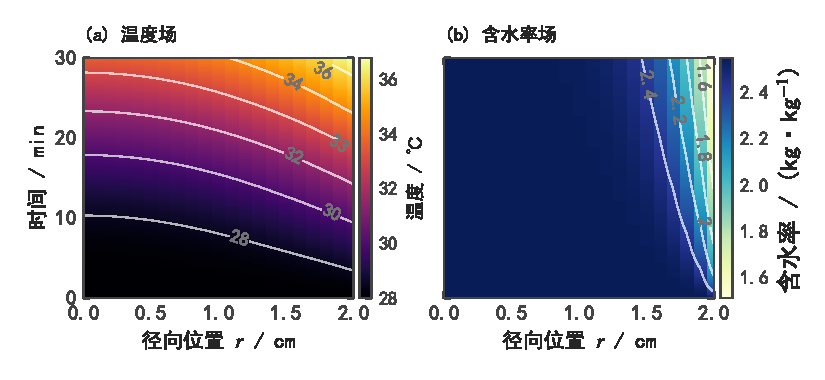
\includegraphics[width=0.9\textwidth,height=0.8\textheight,keepaspectratio]{../figures/fig_field_heatmap_p1.pdf}
  \caption{问题1 温度场（左）与含水率场（右）在预热阶段的时空演化}
  \label{fig:field_heatmap_p1}
\end{figure}

由图~\ref{fig:field_heatmap_p1} 可见，温度扰动自表面向轴心推进，$1800\,\mathrm{s}$ 时轴心温度
仅由 $28\,^{\circ}\mathrm{C}$ 升到约 $33.6\,^{\circ}\mathrm{C}$，尚未达到热风温度，印证预热阶段的特征时间
$\tau_{\mathrm{th}}\approx2369\,\mathrm{s}$ 与观测时窗相当、升温未完成。含水率场则几乎只在近表面
薄层内下降，轴心含水率仍保持在 $C_0=2.55$。径向剖面见图~\ref{fig:radial_profiles}。

\begin{figure}[H]
  \centering
  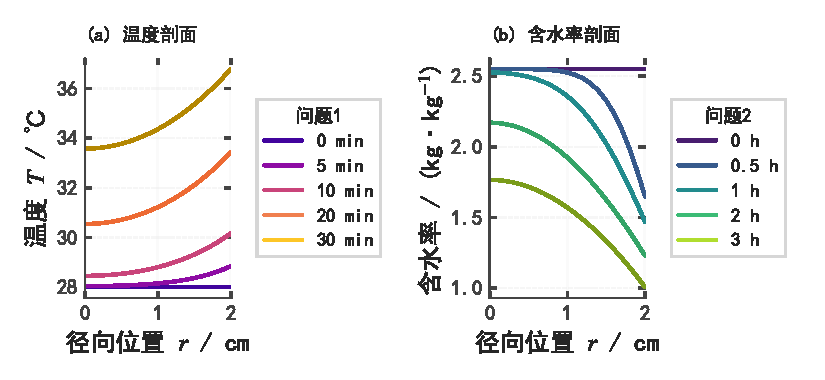
\includegraphics[width=0.9\textwidth,height=0.8\textheight,keepaspectratio]{../figures/fig_radial_profiles.pdf}
  \caption{问题1 不同时刻温度剖面（左）与问题2 含水率剖面（右）的径向分布}
  \label{fig:radial_profiles}
\end{figure}

图~\ref{fig:radial_profiles} 左侧的温度剖面显示 $1800\,\mathrm{s}$ 时沿半径由轴心到表面为
$33.58$,\allowbreak\,$33.77$,\allowbreak\,$34.37$,\allowbreak\,$35.36$,\allowbreak\,$36.79\,^{\circ}\mathrm{C}$，呈单调升高的边界层型分布；对应含水率由轴心
到表面为 $2.5500$,\allowbreak\,$2.5496$,\allowbreak\,$2.5376$,\allowbreak\,$2.3763$,\allowbreak\,$1.5125$，即\textbf{只有最外一到两层含水率明显下降，
轴心几乎未失水}。这说明预热阶段传质被限制在表面薄层，内部尚未"感知"到干燥，也解释了
为何该阶段不宜用于反演内部含水率——内部信息尚未从边界传入。问题一的结果构成后续变物性、
时变边界与移动边界模型的基准解，各问最终数值汇总见表~\ref{tab:main_results}。
